\documentclass[preprint,12pt]{elsarticle}
\usepackage{amssymb}
\usepackage{amsmath}
\usepackage{float}
\usepackage{listings}
\usepackage{amssymb}
\usepackage{tabularx}
\usepackage{tikz}
\usepackage{float}
\usepackage{mathtools}
%\usepackage{minted}
\usepackage[colorinlistoftodos]{todonotes}
\usepackage[ruled,vlined]{algorithm2e}
\usepackage{hyperref}
\usepackage{enumerate}
\usepackage[shortlabels]{enumitem}
\usepackage{amssymb}
\usepackage{subfig}
\usepackage{makecell}
\usepackage{array}
\usepackage{multirow}
\usepackage{mathpazo}
%\usepackage{multicol}
%\usepackage{siunits}
\usepackage{siunitx}
\usepackage{graphicx}
\usepackage{longtable}
\usepackage[toc,page]{appendix}
\usepackage{booktabs}
\usepackage{tabularx}
\usepackage{adjustbox}
\usepackage[section]{placeins}
\usepackage{pdflscape}
\usepackage[utf8]{inputenc}
\usepackage[T1]{fontenc}

\usepackage{natbib}
\bibliographystyle{unsrtnat}


\setlength{\marginparwidth}{4cm}
\usepackage{todonotes}
\newcommand{\inner}[2]{\langle #1 | #2 \rangle}
\newcommand{\R}{\mathbb{R}}
\newcommand{\wij}{W_{ij}}
\newcommand{\loss}{\mathcal{L}}

\journal{Nuclear Instruments and Methods
in Physics Research Section A: Accelerators, Spectrometers,
Detectors and Associated Equipment}

\begin{document}

\begin{frontmatter}

%% \title{Title\tnoteref{label1}}
%% \tnotetext[label1]{}
%% \author{Name\corref{cor1}\fnref{label2}}
%% \ead{email address}
%% \ead[url]{home page}
%% \fntext[label2]{}
%% \cortext[cor1]{}
%% \address{Address\fnref{label3}}
%% \fntext[label3]{}

\title{Latent Variable Clustering for Classification of Events in the AT-TPC}

%% use optional labels to link authors explicitly to addresses:
%% \author[label1,label2]{}https://www.overleaf.com/project/5e73f990fcbd310001959b01
%% \address[label1]{}
%% \address[label2]{}

\author{R.~Solli}
\address{Department of Physics, University of Oslo, POB 1048 Oslo, N-0316 Oslo, Norway}

\author{D.~Bazin}
\address{Department of Physics and Astronomy and Facility for Rare Ion Beams and National Superconducting Cyclotron Facility, Michigan State University, East Lansing, MI 48824, USA}
\author{M.P.~Kuchera}
\address{Physics Department, Davidson College, Davidson, North Carolina, USA}
\author{M.~Hjorth-Jensen}
\address{Department of Physics and Astronomy and Facility for Rare Ion Beams and National Superconducting Cyclotron Facility, Michigan State University, East Lansing, MI 48824, USA}
\address{Department of Physics and Center for Computing in Science Education, University of Oslo, POB 1048 Oslo, N-0316 Oslo, Norway}
\ead{hjensen@frib.msu.edu}
\ead[url]{http://mhjgit.github.io/info/doc/web/}


\begin{abstract}
In this work we introduce the application of convolutional autoencoder neural networks to the analysis of two-dimensional projections of particle tracks from a resonant proton scattering experiment on ${}^{46}$Ar. 
The data we analyze were recorded by an active target time-projection chamber (AT-TPC). Machine learning presents an interesting avenue for researchers operating an AT-TPC, as traditional analysis methods of AT-TPC data are both computationally expensive and fit all particle tracks against the event type of interest. The latter presents a considerable challenge when the space of reactions is not known prior to the analysis. 

We explore the performance of the autoencoder neural networks and a pre-trained VGG16 \cite{Simonyan2014} convolutional neural network on two tasks: a semi-supervised classification task and the unsupervised clustering of particle tracks. On the semi-supervised task, we find that a logistic regression classifier trained on small labelled subsets of the latent space of these models perform very well. On simulated data these classifiers achieve an $f1$ score \cite{Chinchor1992} of $f1>0.95$. The VGG16 latent classifier achieves this result with as few as $N=100$ samples, as does the convolutional autoencoder when trained on the VGG16 representations of the particle tracks. On real data, pre-processed with noise filtering, the same models achieve an $f1>0.7$. For unfiltered real data the models achieve an $f1$ value larger than $0.6$. Both of the previous results were found with the classifiers trained on $N=100$ samples. Furthermore, we found that the autoencoder model reduces the variability in the identification of proton events by $64\%$ from the benchmark logistic regression classifier trained on the VGG16 latent space on real experimental data. 

On the clustering task, we found that a $K$-means algorithm applied to the simulated data in the VGG16 latent space forms almost perfect clusters, with an adjusted rand index \cite{Hubert1985} ($ARI$) $ > 0.8$.  Additionally, the VGG16+K-means approach finds high purity clusters of proton events for real experimental data. We also explore the application of neural networks to clustering by implementing a mixture of autoencoders algorithm. With this model we improved clustering performance on the real experimental data from an $ARI = 0.17$ to an $ARI = 0.40$. However, the neural network clustering suffers from stability issues necessitating further investigations into this approach. 

\end{abstract}

%%Graphical abstract
\begin{graphicalabstract}
%\includegraphics{grabs}
\end{graphicalabstract}

%%Research highlights
\begin{highlights}
\item Research highlight 1
\item Research highlight 2
\end{highlights}

\begin{keyword}
%% keywords here, in the form: keyword \sep keyword

%% PACS codes here, in the form: \PACS code \sep code

%% MSC codes here, in the form: \MSC code \sep code
%% or \MSC[2008] code \sep code (2000 is the default)

\end{keyword}

\end{frontmatter}

\section{Introduction}\label{sec:intro}
\begin{itemize}
    \item Overall goals for the AT-TPC
    \item Nuclear physics motivation for clustering-based (unsupervised) methods
    \item Motivation fro ML approach
    
\end{itemize}

\section{Experimental Details} 
(46Ar)
\section{Methods}\label{sec:methods}
\subsection{Why machine learning}

\begin{itemize}
    \item Traditional MC methods fall short in two principal ways:
    \begin{itemize}
        \item The computational cost per event is too large given the size of the data-sets
        \item The broken tracks, noisy environment creates bad fit statistics for otherwise useful events. End result is $f1 \sim 0.7 $
    \end{itemize}
\end{itemize}

\subsection{Machine Learning}

\begin{itemize}
    \item Reiterate the aim of unsupervised  clustering of events.
    \item Challenges from a machine learning perspective. 
    \begin{itemize}
        \item Supervised vs. Unsupervised learning
        \item Traditional unupervised - distances in high dimensional spaces etc. 
    \end{itemize}
    \item Digression here to explain some ML concepts? Link back to Conv part of Michelles paper? 
    \item Opportunities presented by: 
    \begin{itemize}
        \item Transfer learning (train on VGG use on AT-TPC)
        \item Compression is understanding (leverage autoencoders) 
    \end{itemize}
    \item Building on Kuchera et. al we investigate the VGG16 networks application. 
    \item Novel contribution by applying clustering autoencoder networks. 
\end{itemize}

\subsubsection{Pre-trained neural networks}

Following the previous work of \citet{Kuchera2019}, we will consider representations of our events through the lens of a pre-trained network. In the Machine Learning community, it is not uncommon to publish packaged models with fitted parameters from image recognition contests. These models are trained on datasets with millions of images and classify between hundreds of distinct classes; one such is the imagenet dataset. In their work, \citet{Kuchera2019} use the VGG16 architecture trained on imagenet to classify AT-TPC events very successfully.  We will build on the understanding of using these pre-trained networks in event classification by using VGG16 as an element in the end-to-end training of autoencoders. 

The VGG16 network is one of six analogous networks proposed by \citet{Simonyan2014}, and they were runners up in the ISLVRC(ImageNet large scale visual recognition competition) of 2014 \cite{Russakovsky2015}. The network architectures are fairly simple; for VGG16, there are sixteen layers in the network. The first thirteen of which are convolutional layers with exclusively $3 \times 3$ kernels. The choice of the kernel size is based on the fact that a stacked $3 \times 3$ kernel is equivalent to larger kernels in terms of the receptive field of the output. Three $3 \times 3$ kernels with stride $1$ have a $7 \times 7$ receptive field, but the larger kernel has $81\%$ more parameters and only one non-linearity \cite{Simonyan2014}. Stacking the smaller kernels then contributes to a lower computational cost. Additionally, there is a regularizing effect from the lowered number of parameters and increased explanatory power from the additional non-linearities. The full architecture is detailed in appendix \ref{tab:vgg}.


\subsubsection{Deep clustering: Mixture of autoencoders}\label{sec:mixae}

Another way of representing the clusters is by having multiple latent spaces representing the underlying manifolds that describe each class. This is the central idea in the Mixture of autoencoders (MIXAE) algorithm, introduced by  \cite{Zhang}. To ensure that each autoencoder represents a cluster, we attach a soft-max classifier to the set of latent samples. Recall from equation \ref{eq:softmax} that the soft-max function transforms a network output to a prediction of relative confidences. This classifier assigns a cluster to each autoencoder, coupling the latent space and the reconstructions. The soft-max classifier is trained to output cluster probabilities and penalized for collapsing to assigning one cluster only. The remaining task is then to connect the cluster assignments to the autoencoder reconstructions. This is achieved by multiplying by the cluster confidence with the reconstruction error of each autoencoder.

\begin{figure}[tb]
	\centering
	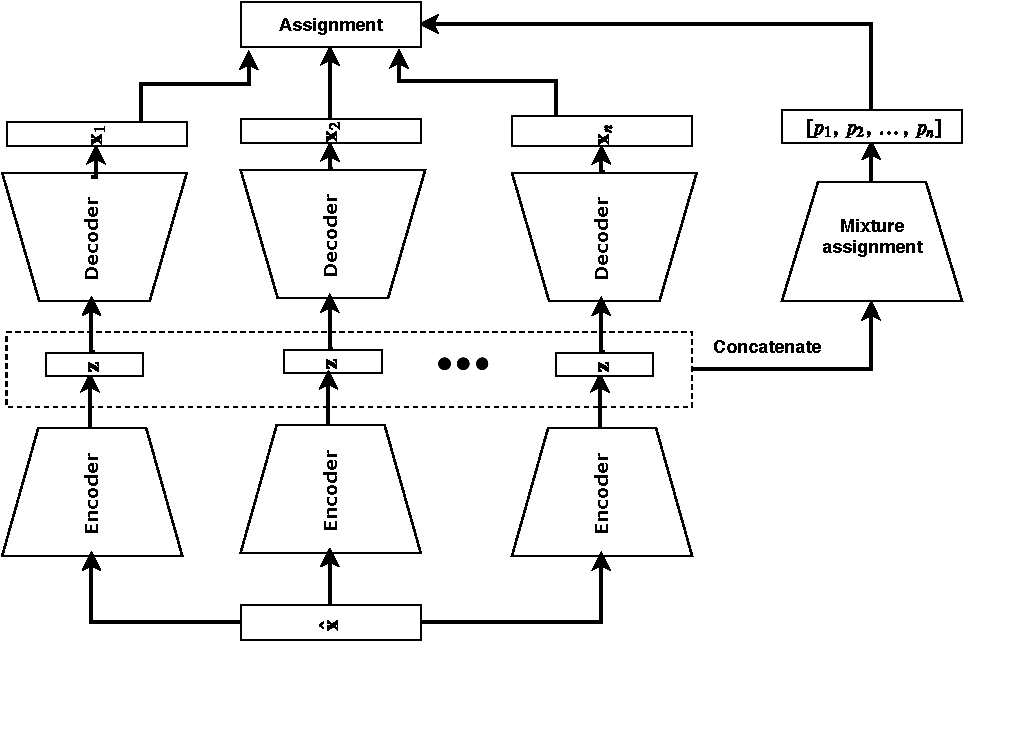
\includegraphics[width=\textwidth]{plots/mixae.pdf}
	\caption[Deep convolutional embedded clustering schematic]{Schematic of a DCEC model. A sample $\hat{\boldsymbol{x}}$ is compressed to set of lower-dimensional representations $\{\boldsymbol{z}^{(i)}\}$ by $N$ autoencoders. These samples are concatenated and passed through an auxiliary assignment network that predicts a confidence of cluster belonging for each autoencoder. For further details see the text. Figure adapted from \citet{Zhang}}
	\label{fig:mixae}
\end{figure}


More formally let $\{\boldsymbol{z}_j^{(i)}\}^N$ be the set of $N$ latent samples from each of the $N$ auto-encoders from a single sample image $\hat{\boldsymbol{x}}^{(i)} \in \R ^{t\times v}$ with height $t$ and width $v$. Furthermore, let the soft cluster assignments be given as $\{p_j^{(i)}\}^N$ and the reconstructed samples be given as $\{\boldsymbol{x}_j^{(i)}\}$. The reconstruction loss is then the sum over each autoencoder multiplied with each cluster assignment, i.e.

\begin{equation}\label{eq:mixae_reconst}
\mathcal{L}_x = \sum_j p_j^{(i)} \mathcal{C}(\boldsymbol{x}_j^{(i)}, \hat{\boldsymbol{x}}^{(i)}),
\end{equation}

\noindent where $\mathcal{C}(\cdot)$ is a cost function like the mean squared error or a cross-entropy.

We ensure that the soft cluster assignments encourage clustering by adding two terms to the total loss. The first is a simple entropy term which, when minimized, encourages the assignments to be one-hot vectors. Mathematically this loss can then be written as the entropy $S(\cdot)$ of a cluster assignment $\boldsymbol{p}$

\begin{equation}\label{eq:mixae_sample}
S(\boldsymbol{p}^{(i)})_{\text{sample}} = -\sum_j p_j^{(i)} \log p_j^{(i)}. 
\end{equation}

\noindent The last ingredient in the loss is then the term which discourages the trivial solution where only one cluster is being assigned. This loss is a batch-wise entropy term, given a mini-batch of $\beta$ samples the loss is computed as 

\begin{equation}\label{eq:mixae_batch}
\begin{split}
S(\{\boldsymbol{p}^{(i)}\}_i)_{\text{batch}}&= \left(-\sum_j \bar{p}_j \log \bar{p}_j \right)^{-1},\\
\bar{\boldsymbol{p}} &= \frac{1}{\beta} \sum_i ^\beta \boldsymbol{p}^{(i)} .
\end{split}
\end{equation}

\noindent The negative exponent in equation \ref{eq:mixae_batch} owes to the fact that we want to maximize the batch-wise entropy.

From equations \ref{eq:mixae_reconst}, \ref{eq:mixae_sample}, and \ref{eq:mixae_batch} we can then compose the full loss for the MIXAE model. \cite{Zhang} note that the optimization depends heavily on the weighting of the different terms and so we introduce the weighting hyperparameters $\alpha$, $\gamma$ and $\theta$, and write the total loss over a mini-batch as 

\begin{equation}\label{eq:mixae_loss}
\begin{split}
\mathcal{L}_{\text{total}}(\{\hat{\boldsymbol{x}}^{(i)}\}^\beta_i) = \frac{1}{\beta}\sum_i \Big( &\frac{t\cdot v}{\theta} \mathcal{L}_x(\boldsymbol{p}^{(i)},\,\boldsymbol{x}^{(i)},\, \hat{\boldsymbol{x}}^{(i)} ) \\
&+ \alpha S(\boldsymbol{p}^{(i)})_{\text{sample}} \Big) \\
&+\gamma S(\{\boldsymbol{p}^{(i)}\}_i)_{\text{batch}}.
\end{split}
\end{equation}

\noindent \citet{Zhang} note that this algorithm has a couple of shortcomings. The batch-entropy term encourages the cluster assignments to be uniformly distributed within the classes. However, it does have a second minimum when the assignments are all equally likely. For biased datasets with significant variations in the number of samples in each class, this can create problems for the algorithm. Additionally, the number of clusters are not dynamically computed by the algorithm but hard-coded by the researchers. This can be problematic if the number of cluster are not known prior to analysis.

\section{Results and Discussions}\label{sec:results}
The principal challenge in the AT-TPC experiments that we are trying to solve is the reliance on labelled samples in the analysis as future experiments may not have as visually dissimilar reaction products  as we observe in the ${}^{46}$Ar experiment.  The  ${}^{46}$Ar experiment does, however, provide a useful example where we can then explore unsupervised techniques. In this chapter, we explore the application of clustering techniques to events represented in latent spaces. 

We begin by exploring a naive K-means approach on the latent space of a pre-trained network. Subsequently, we investigate other clustering methods and two autoencoder based clustering algorithms, as outlined in section \ref{sec:deep_clustering}.

\todo{Drop this argument or build it in the ML section?}
This chapter builds on the previous results from semi-supervised classification. We observe that we can construct high-quality latent spaces. These high-quality spaces facilitate an investigation of clustering techniques. 

\todo{Reword this to not contrast against semi-supervised}
The approach for clustering of events is different from the semi-supervised approach in two meaningful ways. First, it is a harder task, as we will demonstrate. The clustering task thus necessitates a more exploratory approach to the problem. Second, as a consequence of the challenge, the focus will be a bit different than for the semi-supervised approach. We will still utilize the same architectures and models starting with a search over the parameter space over which we measure the performance using the adjusted rand score (ARS) and accuracy defined in section \ref{sec:unsupervised_perf} and \ref{sec:supervised_perf}, respectively.

As with chapter  \ref{chap:classification} where we explored the semi-supervised results, we begin this chapter by considering the VGG16 pre-trained model as a benchmark.

Lastly, we note that the focus of this work is mainly on discovering possible avenues for further research. This focus requires a broad scan of possible avenues rather than a rigorous analysis of one specific model.
\subsection{Transfer learning}
As in chapter \ref{ch:architectures}, we also use the VGG16 pre-trained network as a baseline for the clustering performance. We begin by considering a classical K-means approach to clustering. However, the output from the VGG16 network is very high dimensional with output vectors in $\R^{8192}$. \todo{reword} One of the primary concerns is then the curse of dimensionality, where the ratio of distances goes to one with increasing dimensionality as shown by \citet{Aggarwal}. However, one of the central caveats to the authors  finding is that the elements are uniformly distributed in the latent space. It is then possible that all the class information lies in some sub-space of the latent data. To investigate this, we perform clustering analysis using the full representation and the $10^2$ first principal components only. 

\subsection{K-means}

We begin by investigating the K-means clustering algorithm on the VGG16 latent space. As in chapter \ref{chap:classification} the VGG16 model is pre-trained on the imagenet dataset creating a set of vectors $\boldsymbol{x} \in \R^{8192}$. To cluster we use \lstinline{scikit-learn} implementation of the K-means algorithm, with default parameters \cite{Pedregosa2011}. The results of the clustering runs are included in table \ref{tab:clstr_vgg}. We observe that we are able to attain near-perfect clustering on simulated data and that there is a sharp decline in performance as we add noise by moving to the filtered and full datasets. 

\begin{table}[H]
\centering 
\caption[K-means on pre-trained model]{K-means clustering results on AT-TPC event data. We observe that the performance predictably decreases with the amount of noise in the data.}\label{tab:clstr_vgg}
\begin{tabular}{lll}
\toprule
{} & Accuracy &   ARI \\
\midrule
Simulated &     0.97 &  0.89 \\
Filtered  &     0.74 &  0.39 \\
Raw       &     0.59 &  0.17 \\
\bottomrule
\end{tabular}

\end{table}

In addition to the performance measures reported in table \ref{tab:clstr_vgg}, it is interesting to observe which samples are being wrongly assigned. We achieve this by tabulating the assignments of samples relative to their ground truth labels. From these tables, we can infer which classes are more or less entangled with others. We tabulate the results for each dataset is in figure \ref{fig:clster_confmat}. We observe that the proton class is consistently assigned in a pure cluster. Purity is inferred by how much spread there is in the column between the ground truth labels. A high-quality cluster will, in addition to being pure, also capture most entries the class represented by the cluster. For example, consider the row corresponding to the proton class in figure \ref{fig:clster_confmat}. The column corresponding to the largest entry in the proton row has zero other predicted classes in it. From this, we conclude that the proton cluster is a high quality, high purity cluster. 

\begin{figure}
\centering

	\subfloat{
	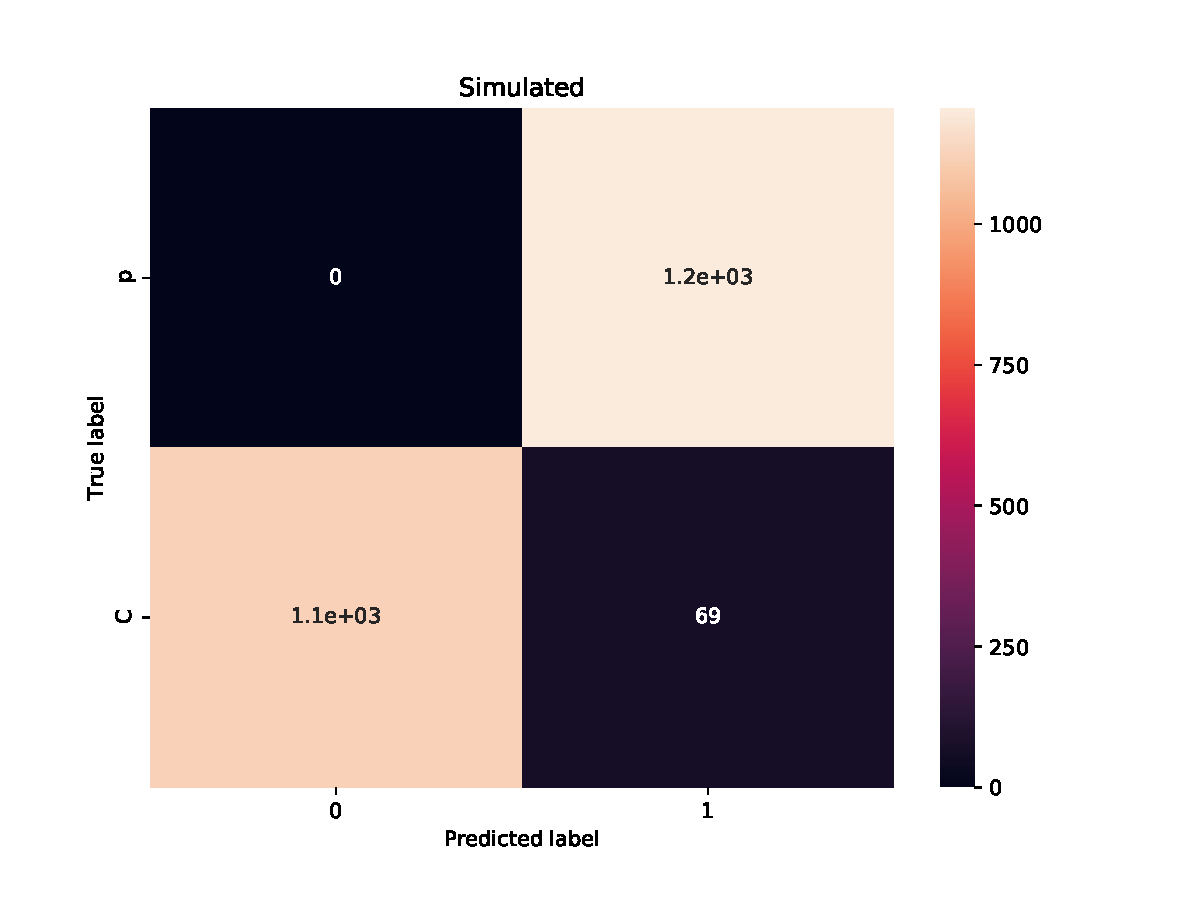
\includegraphics[width=0.35\textwidth]{./plots/Simulatedvgg_pca_conf_mat.pdf}

}
	\hspace{-1cm}
	\subfloat{
	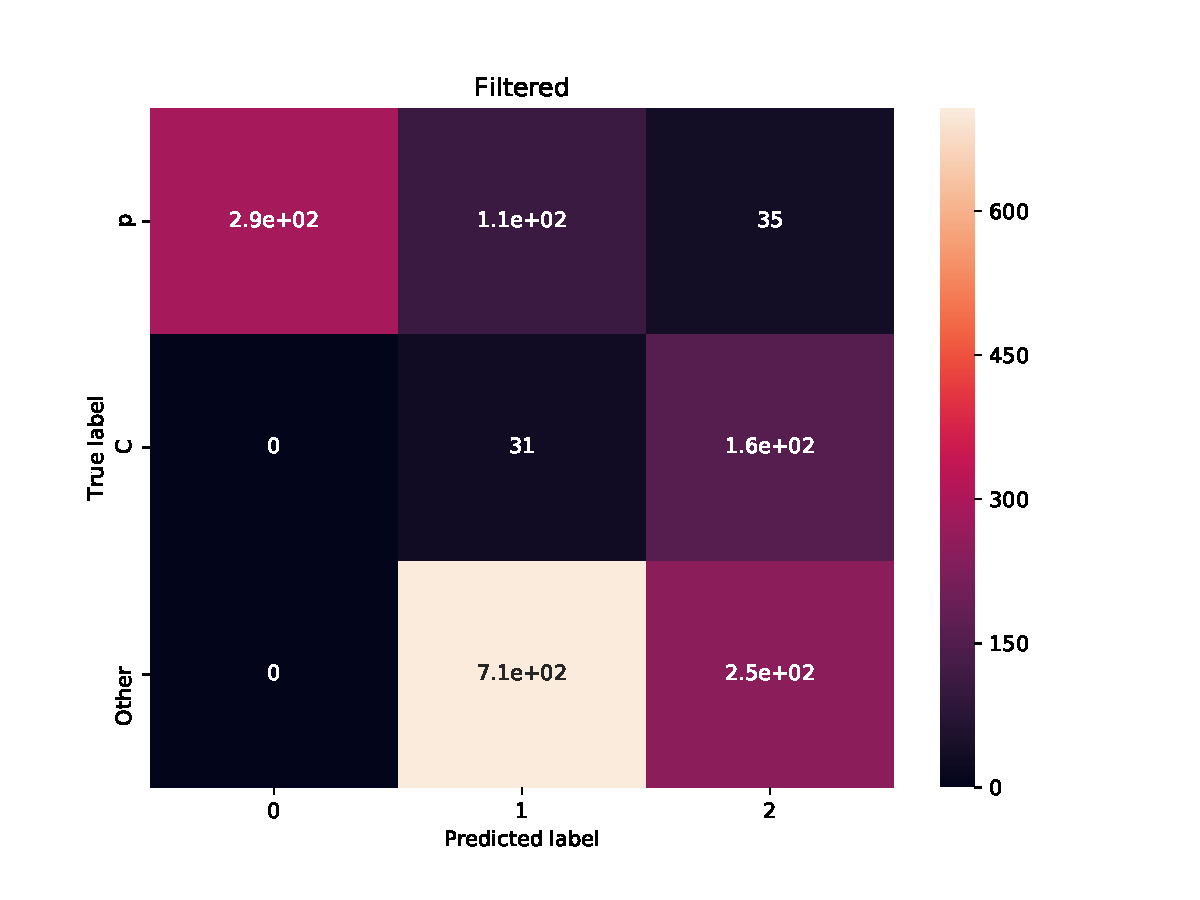
\includegraphics[width=0.35\textwidth]{plots/Filteredvgg_pca_conf_mat.pdf}
}
	\hspace{-1cm}
	\subfloat{
	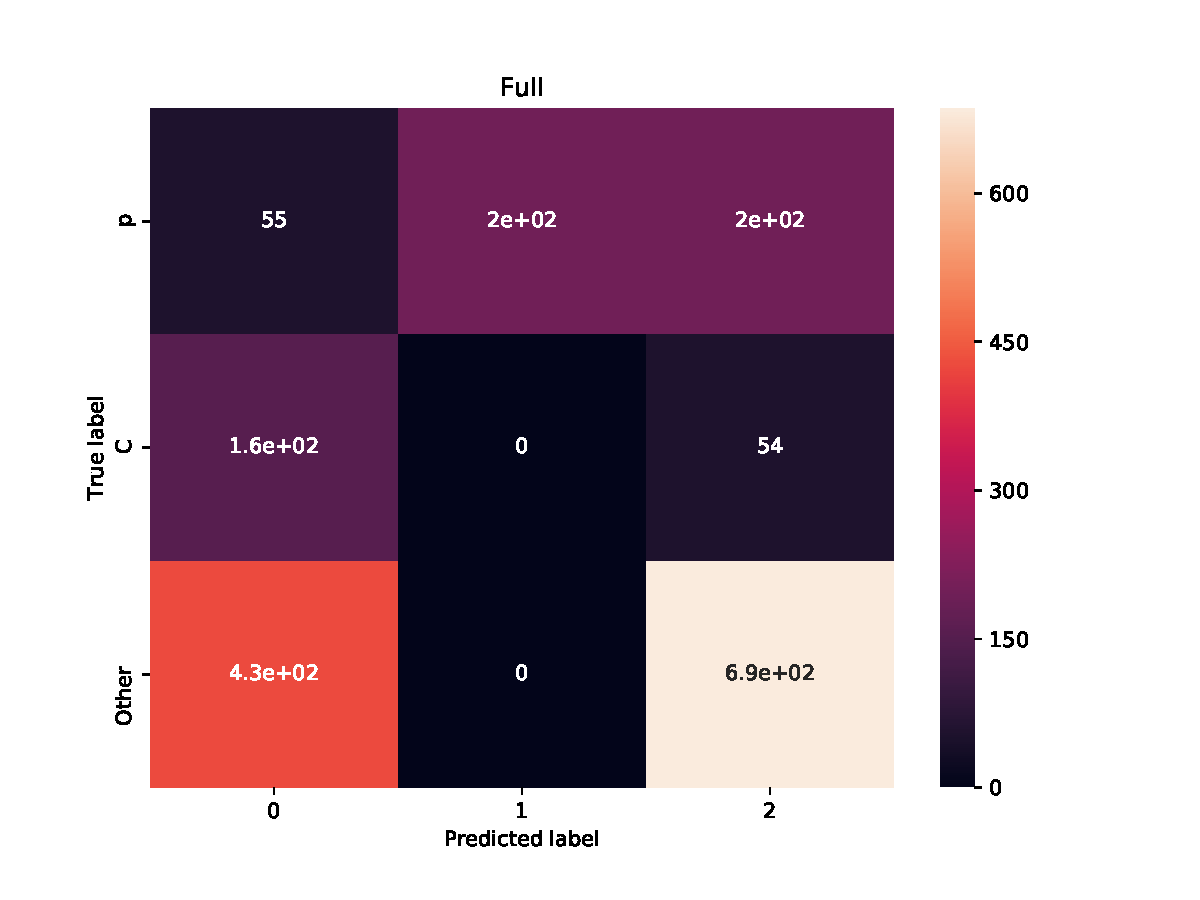
\includegraphics[width=0.35\textwidth]{plots/Fullvgg_pca_conf_mat.pdf}
}
\caption[Pre-trained network - confusion matrices]{Confusion matrices for the K-means clustering of simulated, filtered and full AT-TPC events. The true labels indicate samples belonging to the p (proton), carbon (C), or other classes. }\label{fig:clster_confmat}
\end{figure}

We repeat this analysis using a PCA dimensionality reduction on the latent space of the VGG16 model. This is done to estimate to what degree the class separating information is encoded in the entirety of the latent space, or in some select regions. The results from the PCA analysis were virtually identical to the results sans the PCA, and so we omit them for brevity. 

Furthermore, we wish to characterize further the clusters presented in figure \ref{fig:clster_confmat}. To achieve this, we sample from the proton samples belonging to different clusters for the filtered and full data.

\begin{figure}
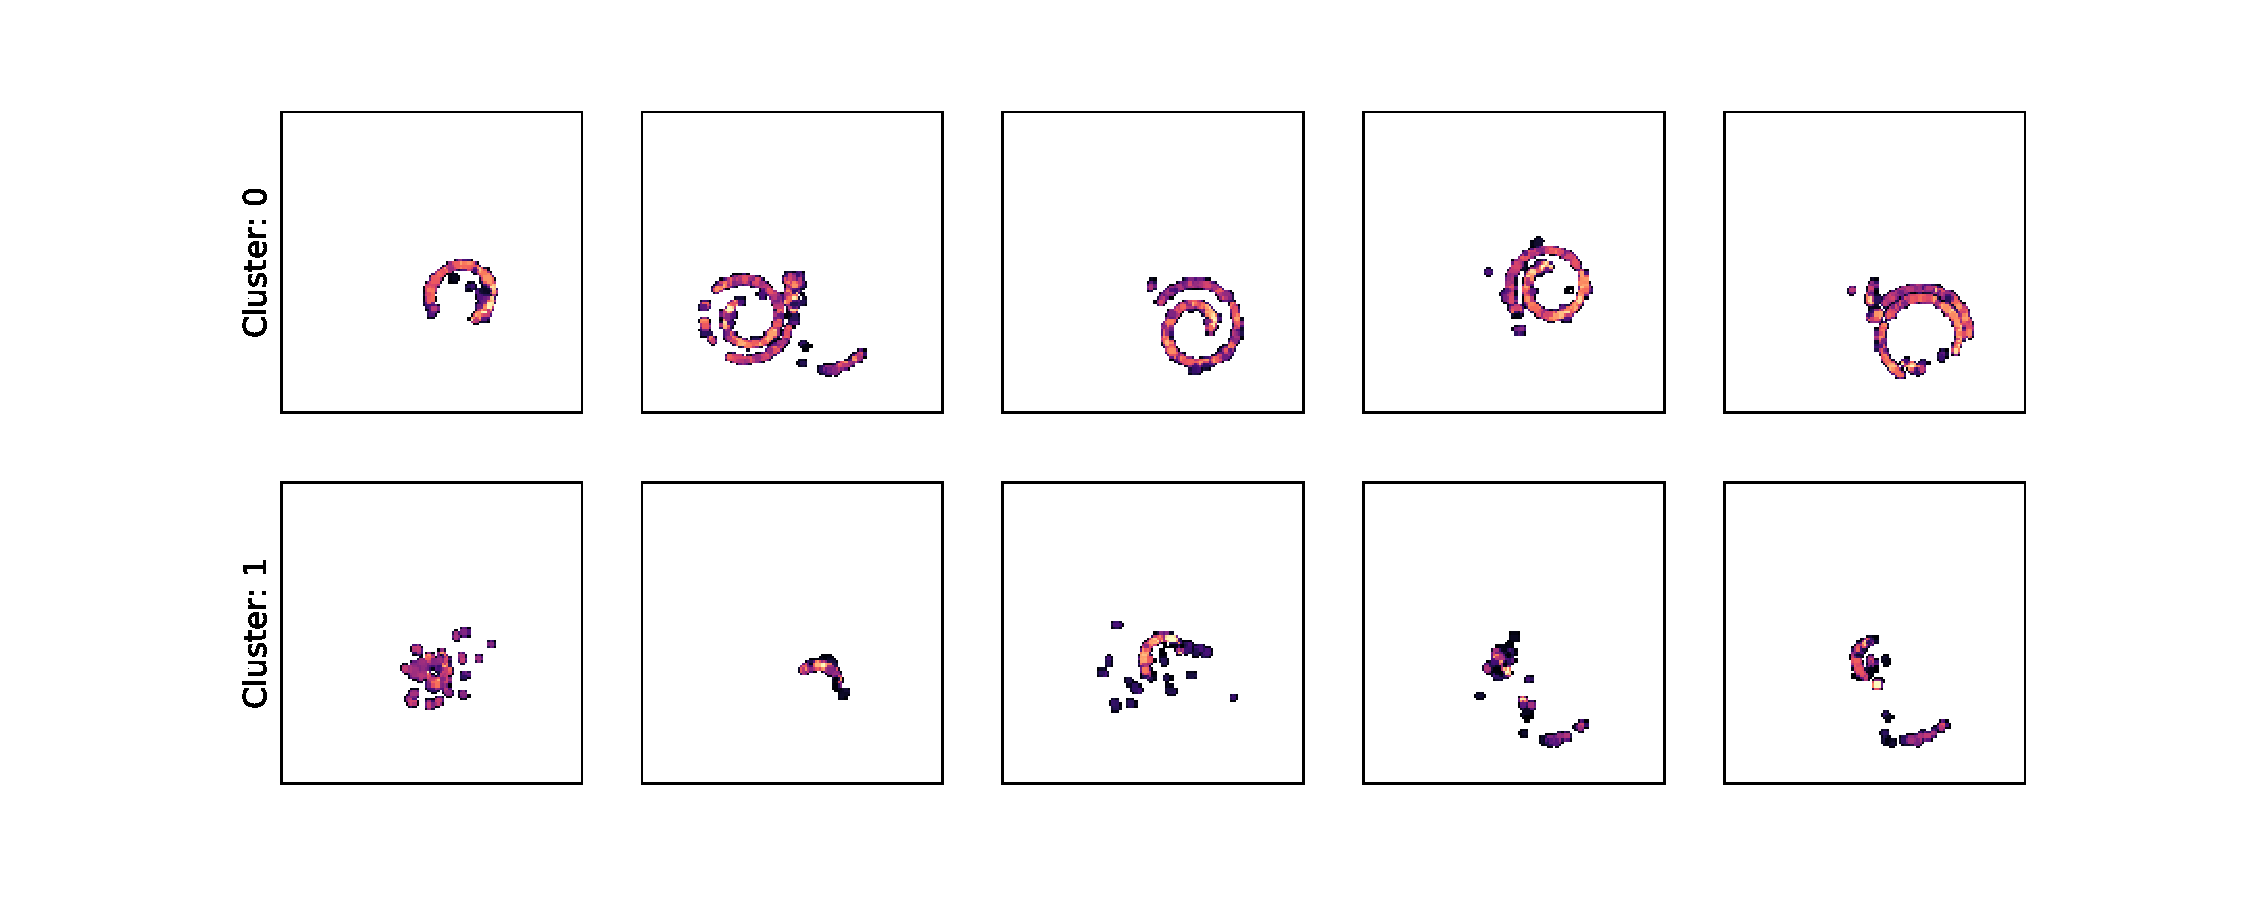
\includegraphics[width=\textwidth]{plots/filtered_vgg_cluster_repr.pdf}
\caption[Filtered proton samples by cluster belonging]{Illustrating a sample of proton events from different K-means clusters from the filtered dataset. Each row belongs to a single cluster corresponding to the filtered confusion matrix in figure \ref{fig:clster_confmat}}\label{fig:filtered_vgg_clster_repr}
\end{figure} 

\begin{figure}
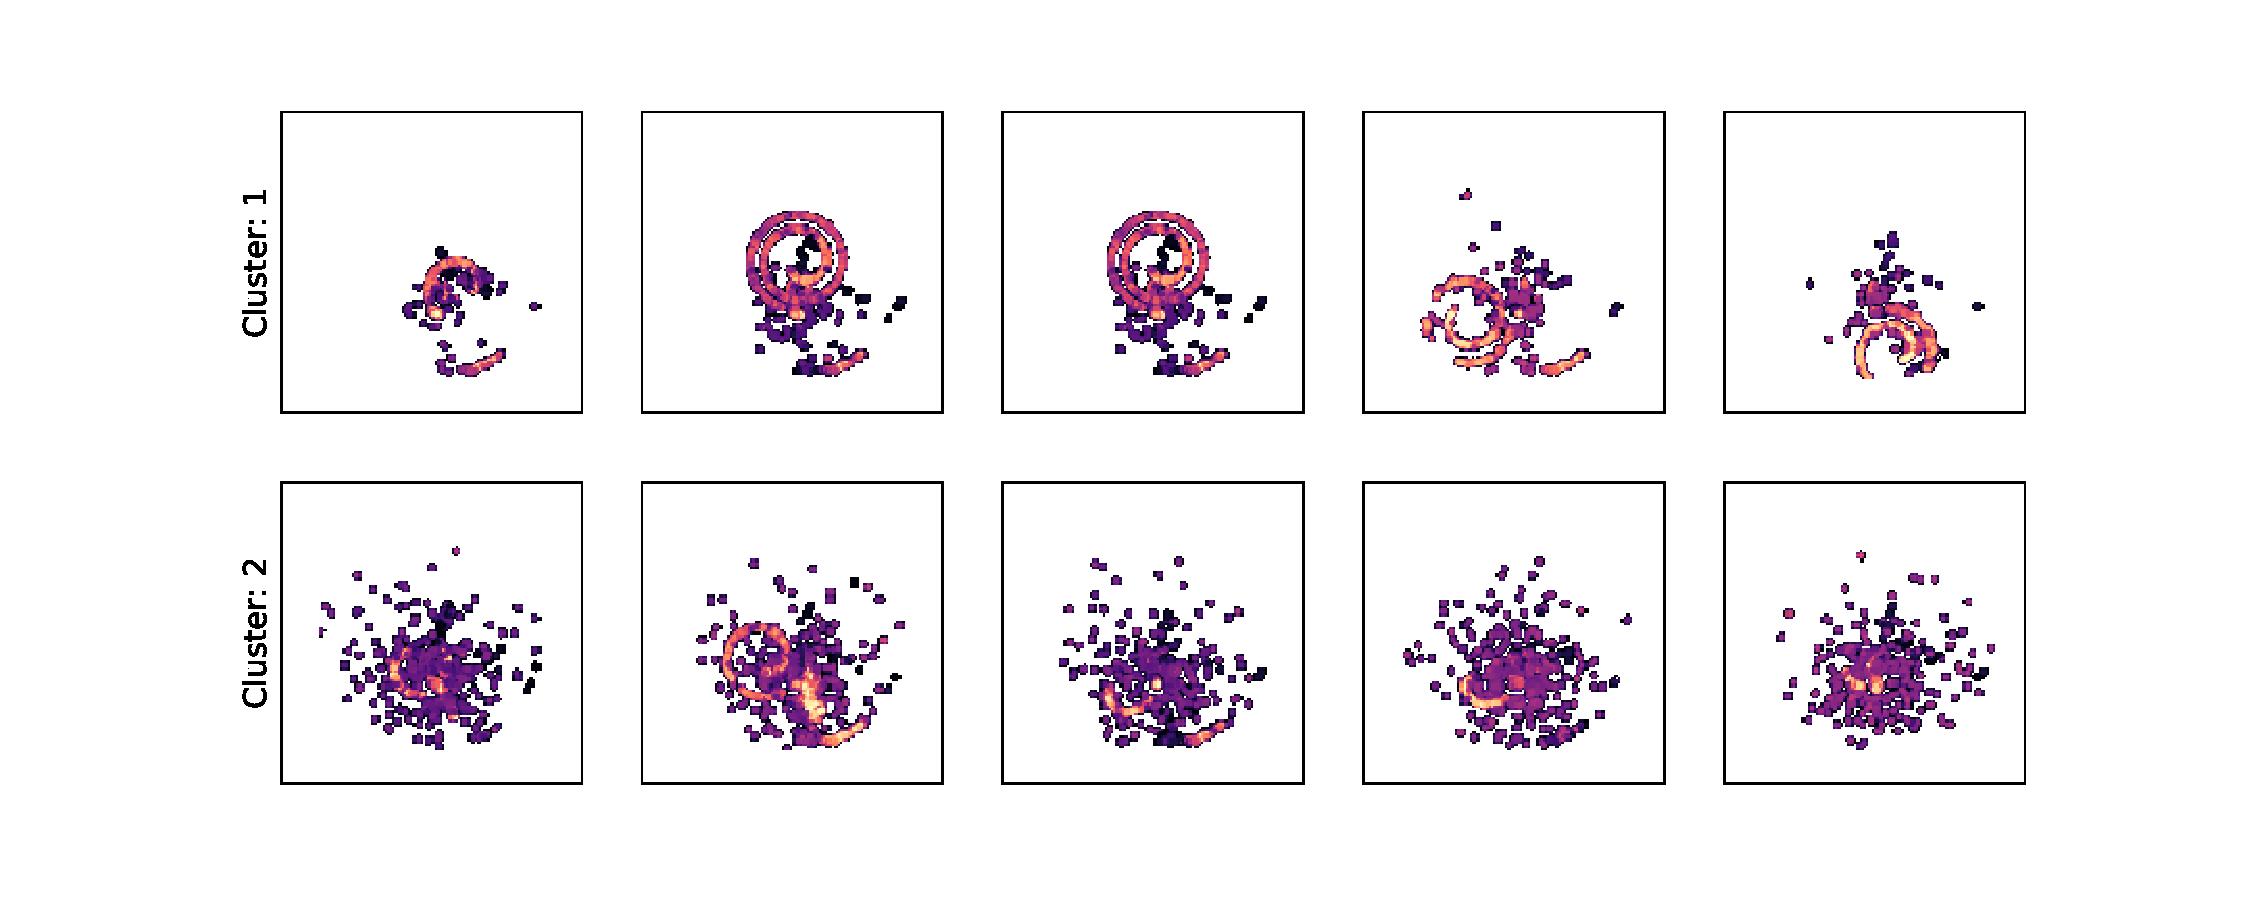
\includegraphics[width=\textwidth]{plots/full_vgg_cluster_repr.pdf}
\caption[Full proton samples by cluster belonging]{Illustrating a sample of proton events from different K-means clusters from the full dataset. Each row belongs to a single cluster corresponding to the full confusion matrix in figure \ref{fig:clster_confmat}}\label{fig:full_vgg_clster_repr}
\end{figure} 

In addition to the results presented in this section, we performed clustering with a number of different algorithms included in the \lstinline{scikit-learn} package. None of them provided any notable differences from the K-means results or were significantly worse. Notably, the DBSCAN algorithm failed to provide any useful clustering results. We find this important as one of the significant drawbacks of K-means, and the deep clustering algorithms presented in section \ref{sec:deep_clustering}, is that they are all dependent on pre-determining the number of clusters. This is not the case for DBSCAN. 
\subsection{Autoencoder clustering}

In the previous section we demonstrated a potential for clustering of events from an AT-TPC experiment. To build on this result we will in this section explore the application of the mixture of autoencoders (MIXAE) algorithm introduced in section \ref{sec:deep_clustering}. The other algorithm introduced in section \ref{sec:deep_clustering}, deep clustering with convolutional autoencoders (DCEC), consistently collapsed to just one cluster for all datasets.

In the MIXAE algorithm the hyper-parameters to adjust are all the ordinary parameters that we introduced in table \ref{tab:convae_hyperparams}. In addition to those parameters we have the weighting of the loss terms: $\theta$, $\alpha$ and $\gamma$. These weighting parameters are attached to the reconstruction loss, sample entropy and batch-wise entropy respectively. \cite{Zhang} note that these parameters are very important for the model performance and so we focus primarily on these. 

\todo{but why}We empirically freeze the convolutional autoencoder hyperparameters to compress the original $128 \times 128$ to a $8 \times 8$ pixel grid using four convolutional layers. The parameters chosen for the autoencoders are listed in full in table \ref{tab:mixe_ae_hyperparams}.

\begin{table}[H]
\todo{prettify or remove}
\renewcommand*{\arraystretch}{0.5}
\centering
\caption{Hyperparameters selected for the autoencoder components of the MIXAE algorithm, see table \ref{tab:convae_hyperparams} for a full description of the parameters.}\label{tab:mixe_ae_hyperparams}
\setlength{\extrarowheight}{15pt}
\hspace*{-0.5in}
\begin{tabular}{ll}
\toprule
Hyperparameter & Value \\
\midrule
\multicolumn{2}{l}{Convolutional parameters: } \\
\midrule
Number of layers & $4$ \\
Kernels & $[3,\,3,\,3,\,3]$\\
Strides & $[2,\,2,\,2,\,2]$ \\
Filters & $[64,\, 32, \,16, \,8,]$ \\ 
\midrule
\multicolumn{2}{l}{Network parameters: } \\
\midrule
Activation & LReLu \\
Latent type & None \\
Latent dimension & 20  \\
$\beta$ & N/A \\
Batchnorm & False \\
\midrule
\multicolumn{2}{l}{Optimizer parameters: } \\
\midrule
$\eta$ & $10^{-3}$ \\
$\beta_1$ & $0.9$ \\
$\beta_2$ & $0.99$ \\
\bottomrule
\end{tabular}
\end{table}

Since there are then only three remaining hyperparameters we choose to perform a coarse grid-search as described in section \ref{sec:hyperparam_search_arch}.

\begin{table}
\centering
\caption{Hyperparameter grid for the MIXAE loss weighting terms. The grid is given as exponents for logarithmic scales.}\label{tab:mixae_loss_weights}
\begin{tabular}{lll}
\toprule
Parameter & Grid & Scale \\
\midrule 
$\theta$ & $[-1,\, 5]$ & Logarithmic \\
$\alpha$ & $[-5,\, -1]$ & Logarithmic \\
$\gamma$ & $[3,\, 5]$ & Logarithmic
\end{tabular}
\end{table}

\subsection{Simulated AT-TPC data}

To train the MIXAE clustering algorithm, we use the large simulated dataset with $M=80000$ points, evenly distributed between proton- and carbon-events. The algorithm is trained on a subset of $60000$ of these samples, and we track performance on the remaining $20000$ events. 

The grids selected for the search are listed in table \ref{tab:mixae_loss_weights}. The search yielded an optimal configuration with 

\begin{align}
\theta = 10^{-1}, \\
\alpha = 10^{-2}, \\
\gamma = 10^5.
\end{align}

Finally, for these parameters we re-ran the algorithm $N=10$ times to investigate the stability of the algorithm. The results are reported in figure \ref{fig:mixae_sim}. We observe that while the algorithm can achieve very strong performance, with an adjusted rand index (ARI) $ > 0.8$, it fluctuates strongly with repeated experiments. The $ARI$ is a clustering performance measure similar to accuracy, but adjusted for chance. We elaborate on the $ARI$ score in section \ref{sec:unsupervised_perf}. As mentioned in section \ref{sec:mixae} the batch-entropy has a second minimum when the cluster confidences are near equal. It is this behavior we observe in figure \ref{fig:mixae_sim}.

\begin{figure}[H]
\centering
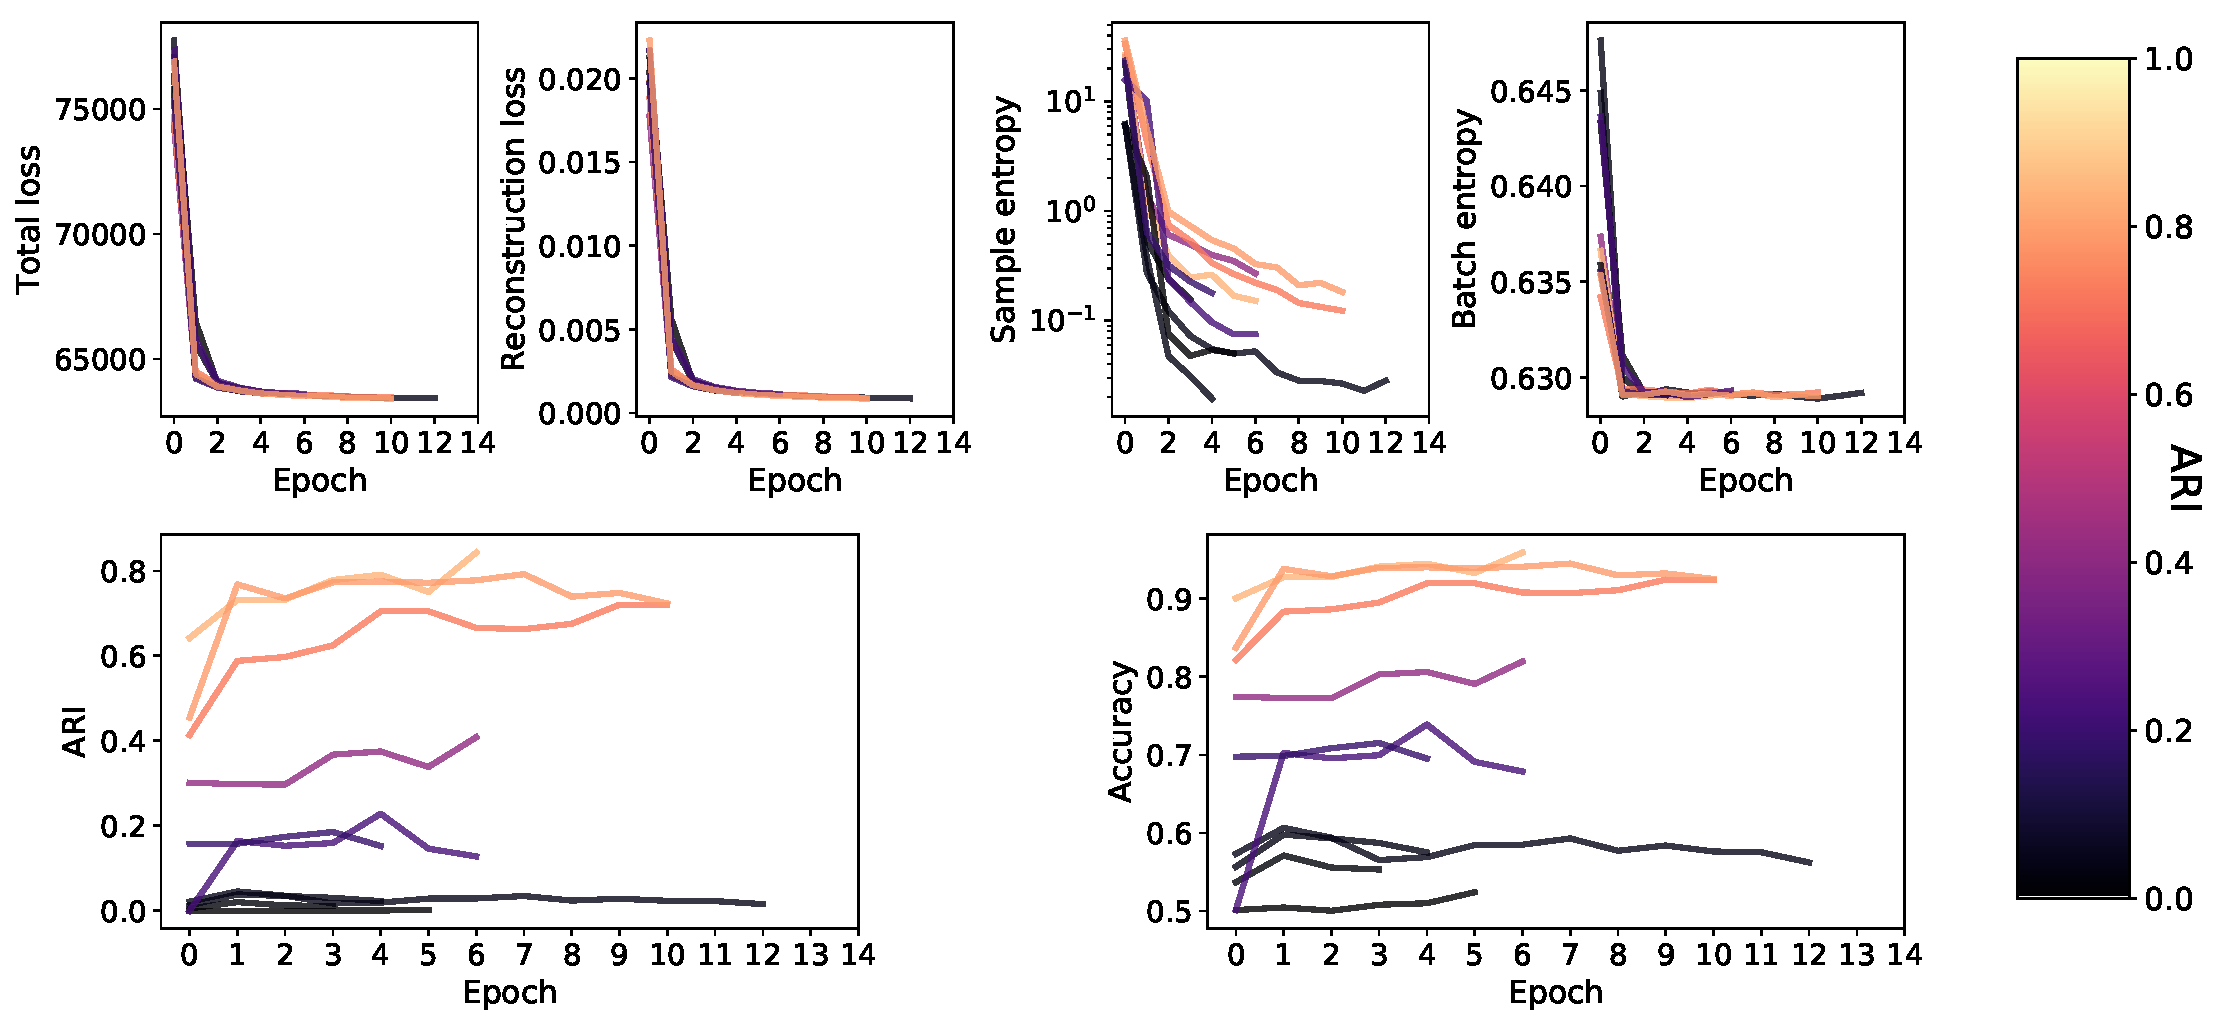
\includegraphics[width=\textwidth]{./plots/sim_mixae.pdf}
\caption[Clustering performance of MIXAE on simulated AT-TPC data]{Performance for the MIXAE model on simulated AT-TPC data. In the top row the loss components are plotted for each run, and in the bottom row the adjusted rand index (ARI) and clustering accuracy are shown. Each run is color-coded with the ARI achieved at the end of the run. }\label{fig:mixae_sim}
\end{figure}

\subsection{Filtered AT-TPC data}

We repeat the optimization steps in the previous section for the filtered AT-TPC data. The exception being that we allow the algorithm to train on the labelled samples. Beginning with a wide grid equal to the grid used for the simulated data we searched over all parameter configurations to find promising values. We then performed a local search around these values to pin-point the hyperparameter configuration. This search yielded the optimal hyper-parameters 

\begin{align}
\theta &= 10^{1}, \\
\alpha &= 10^{-1}, \\
\gamma &= 3.162\times 10^3.
\end{align}

\noindent The results of the runs are included in figure \ref{fig:mixae_clean}. We observe ghat the highest performing models reach an $ARI > 0.5$, which is higher than the performance achieved by the K-means algorithm applied to the VGG16 latent space. 

\begin{figure}[H]
\centering
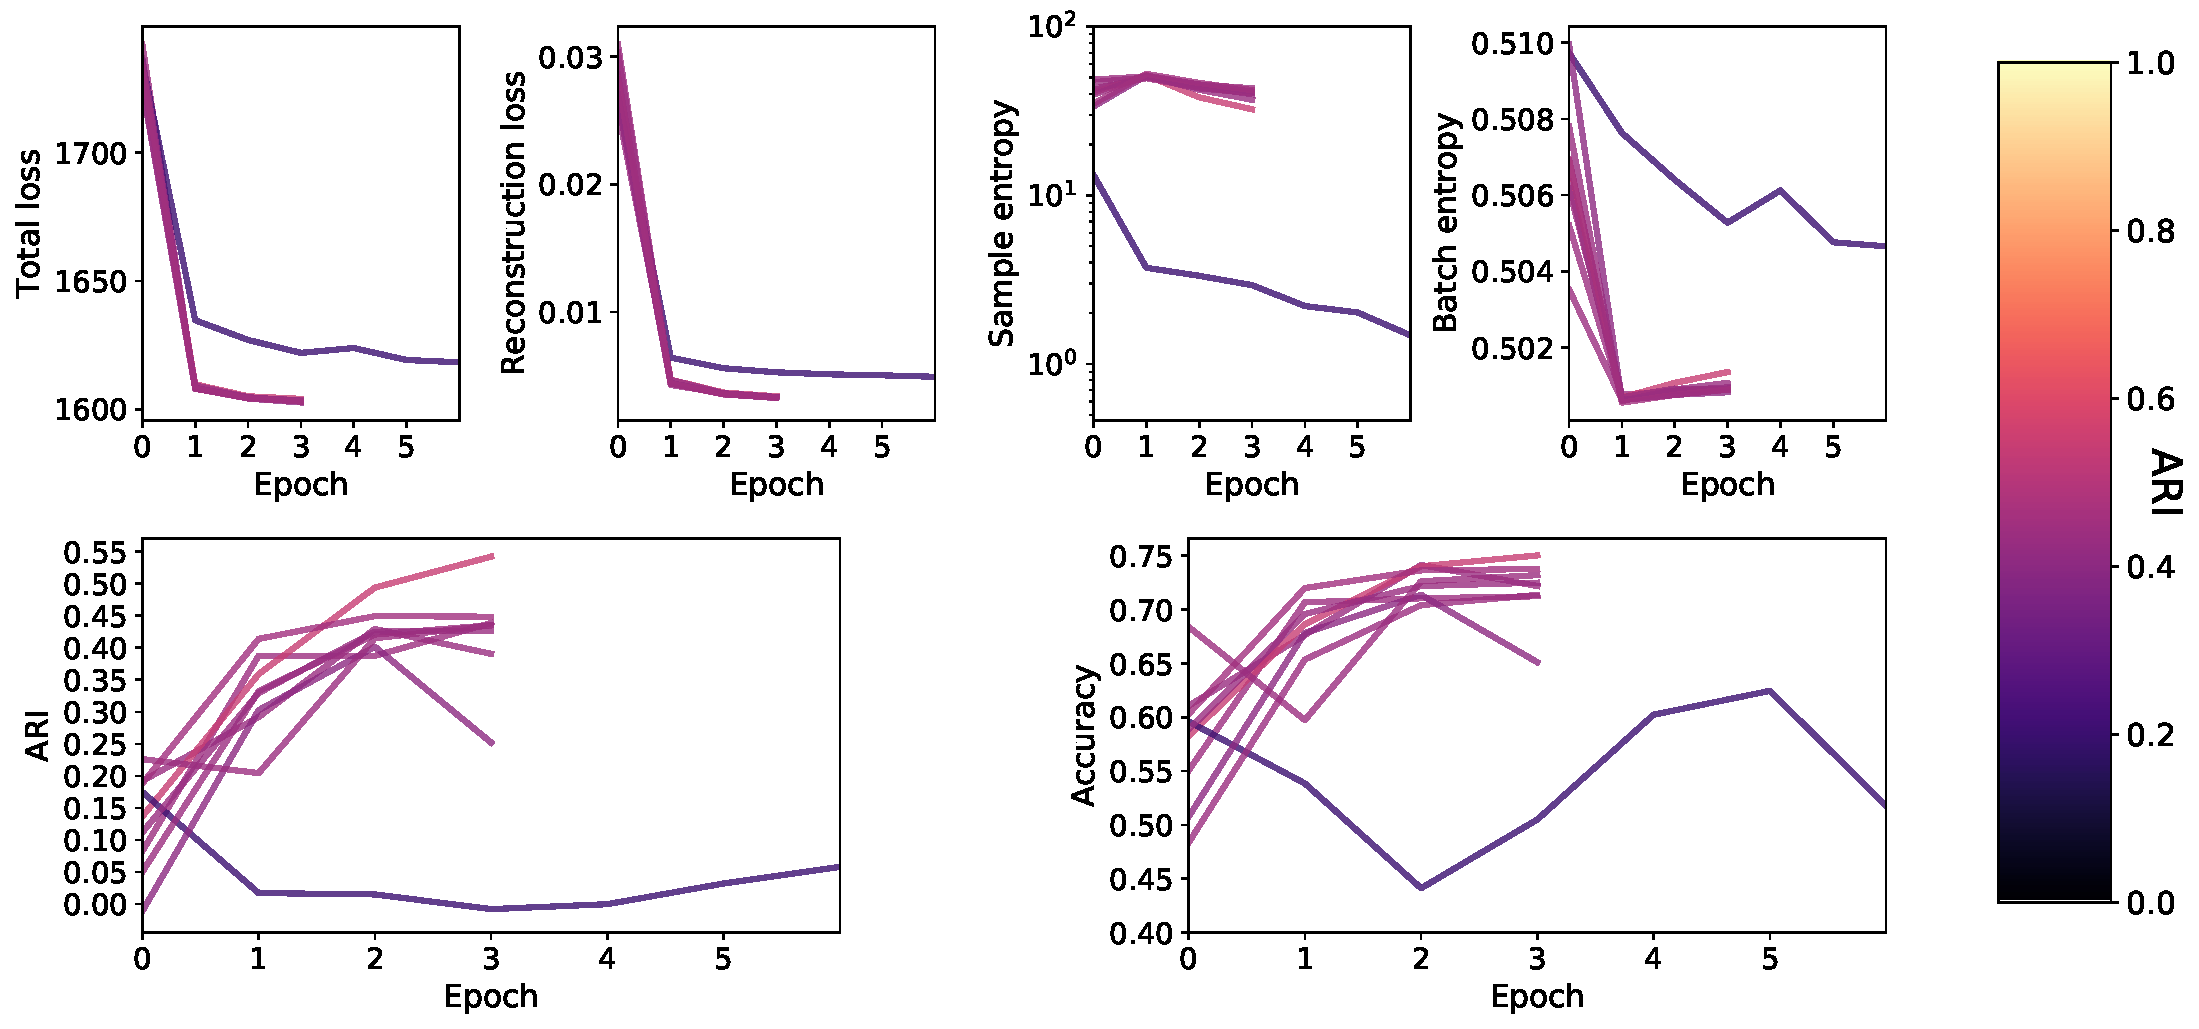
\includegraphics[width=\textwidth]{./plots/clean_mixae.pdf}
\caption[Clustering performance of MIXAE on filtered event AT-TPC data]{Performance for the MIXAE model on filtered AT-TPC data. In the top row the loss components are plotted for each run, and in the bottom row the adjusted rand index (ARI) and clustering accuracy are shown. Each run is color-coded with the ARI achieved at the end of the run.}\label{fig:mixae_clean}
\end{figure}


\subsection{Full AT-TPC data}

As in the two previous sections, we repeat the same procedure of iterative grid searches on the MIXAE loss-weights. Each configuration is re-run a total of $N=10$ times to capture fluctuations in the performance before a final selection is made on the hyperparameters. For the full dataset the MIXAE hyperparameters converge to the same values as for the clean data, i.e. 


\begin{align}
\theta &= 10^{1}, \\
\alpha &= 10^{-1}, \\
\gamma &= 3.162\times 10^3.
\end{align}

\noindent As with the previous datasets we include a plot of the loss curves and performance measures for $N=10$ runs with the same loss-weight parameters, shown in figure \ref{fig:mixae_full}.

\begin{figure}[H]
\centering
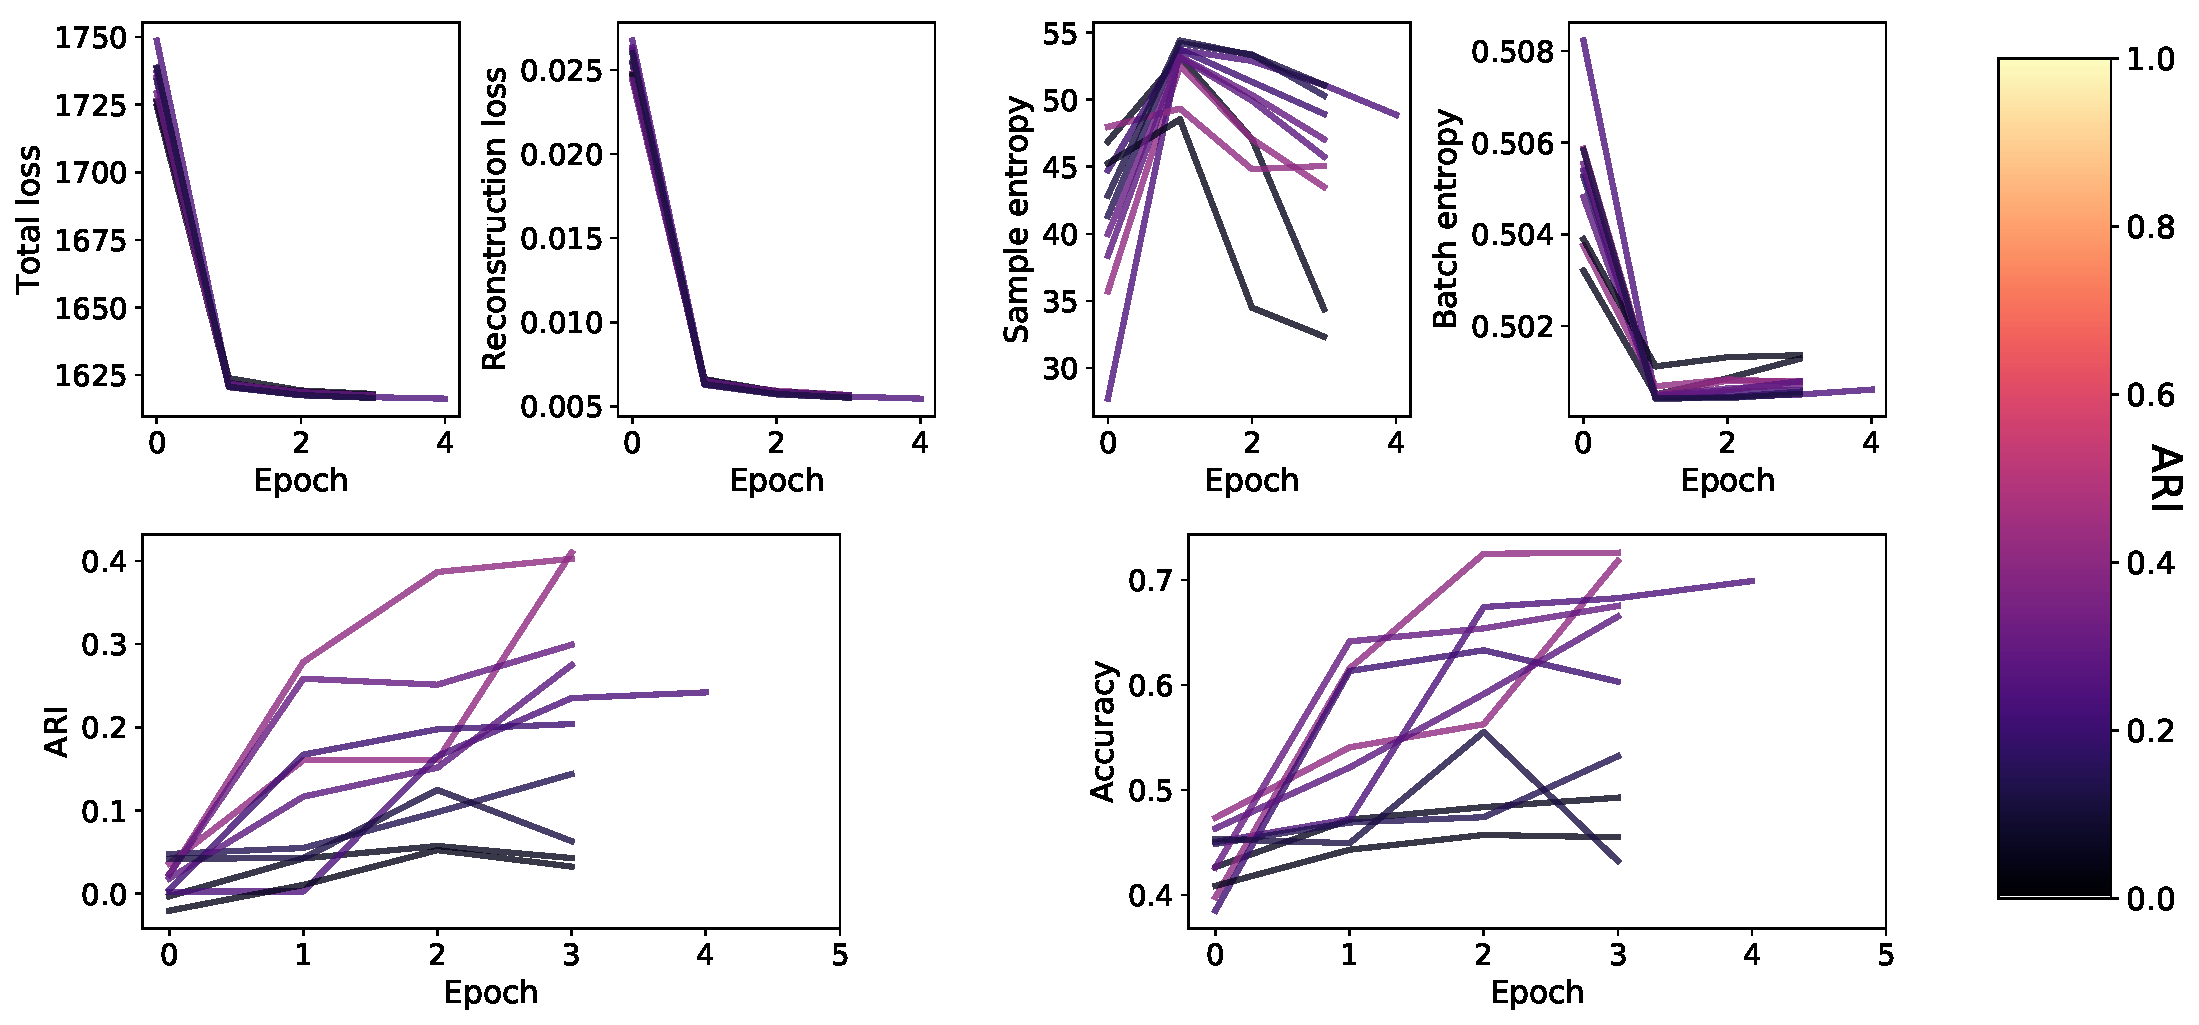
\includegraphics[width=\textwidth]{./plots/real_mixae.pdf}
\caption[Clustering performance of MIXAE on full event AT-TPC data]{Performance for the MIXAE model on un-filtered AT-TPC data. In the top row the loss components are plotted for each run, and in the bottom row the adjusted rand index (ARI) and clustering accuracy are shown. Each run is color-coded with the ARI achieved at the end of the run.}\label{fig:mixae_full}
\end{figure}

\subsection{Comparing performance}

It is also interesting to compare and contrast the clustering results from the MIXAE model with those of the VGG16$+$K-means outside the fairly abstract accuracies and rand scores. It is especially interesting to compare the cluster assignments, as they can inform further research efforts in the clustering of AT-TPC events. We illustrate the clustering with confusion matrices that are shown in figure \ref{fig:mixae_confmat}. From these matrices, we observe that the MIXAE applied to the clean data correctly clusters the noise events. Additionally, it identifies two proton clusters. We observe that these proton clusters are both less pure than the VGG16+K-means clusters and that there does not seem to be a visually meaningful difference between these clusters. The latter is inferred from figure \ref{fig:filtered_mixae_clster_repr}. 

Applied to the real data the MIXAE correctly separates the proton class, however it is unable to separate the carbon events from the amorphous noise events or from the proton cluster. 

\begin{figure}[H]
\centering

	\subfloat{
	\includegraphics[width=0.5\textwidth]{plots/filtered_mixae_conf_mat.pdf}
}
	\hspace{-1cm}
	\subfloat{
	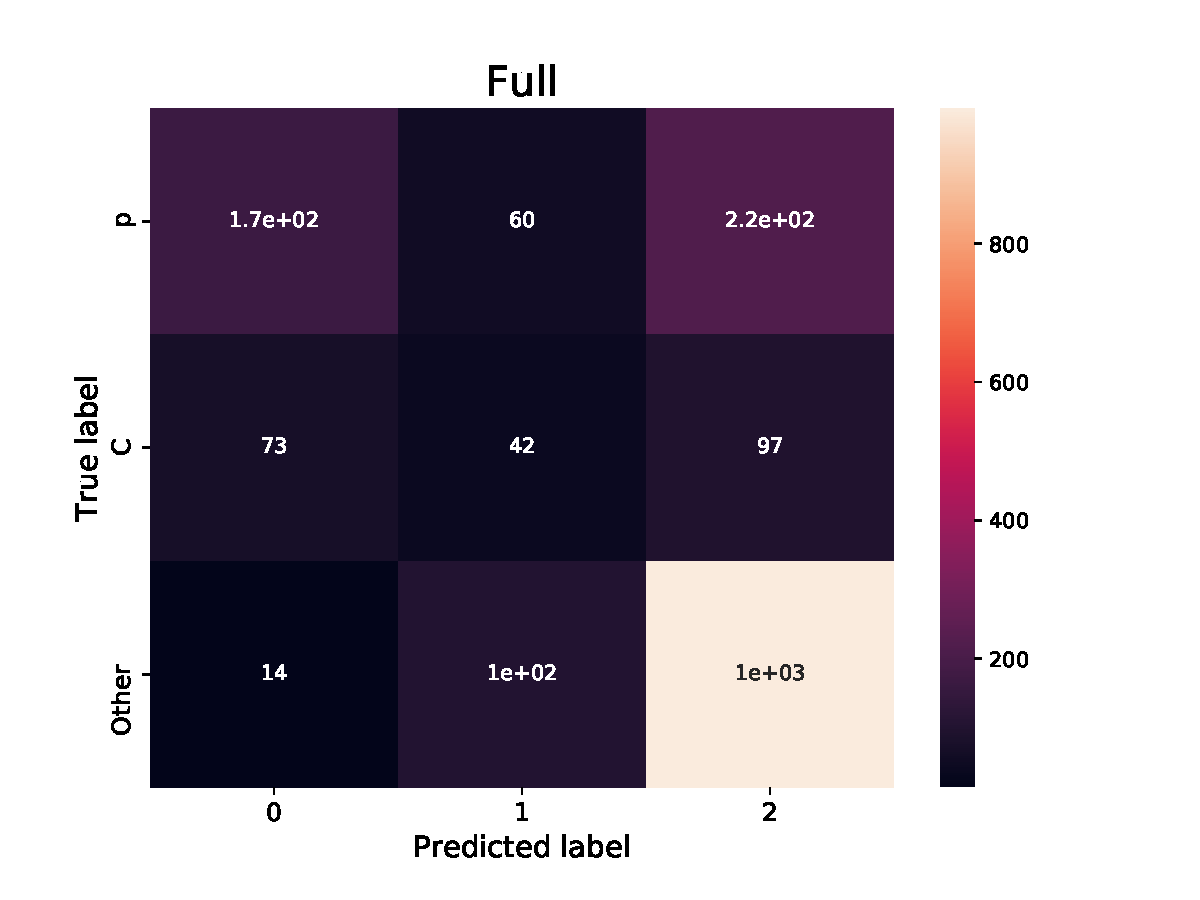
\includegraphics[width=0.5\textwidth]{plots/full_mixae_conf_mat.pdf}
}
\caption[MIXAE - confusion matrices]{Confusion matrices for the MIXAE clustering algorithm on filtered and full AT-TPC events. The true labels indicate samples belonging to the p (proton), carbon (C), or other classes. }\label{fig:mixae_confmat}
\end{figure}

Lastly we wish to further investigate if there are systematic differences between proton events that were placed in different clusters for the clean and full data. From figure \ref{fig:mixae_confmat} we see that the MIXAE algorithm creates two proton clusters for the filtered data, and places about fifty per-cent of the proton events in a cluster with the amorphous "other" events. We extract some proton events from these clusters to inspect whether systematic differences occur. 


\begin{figure}
\centering
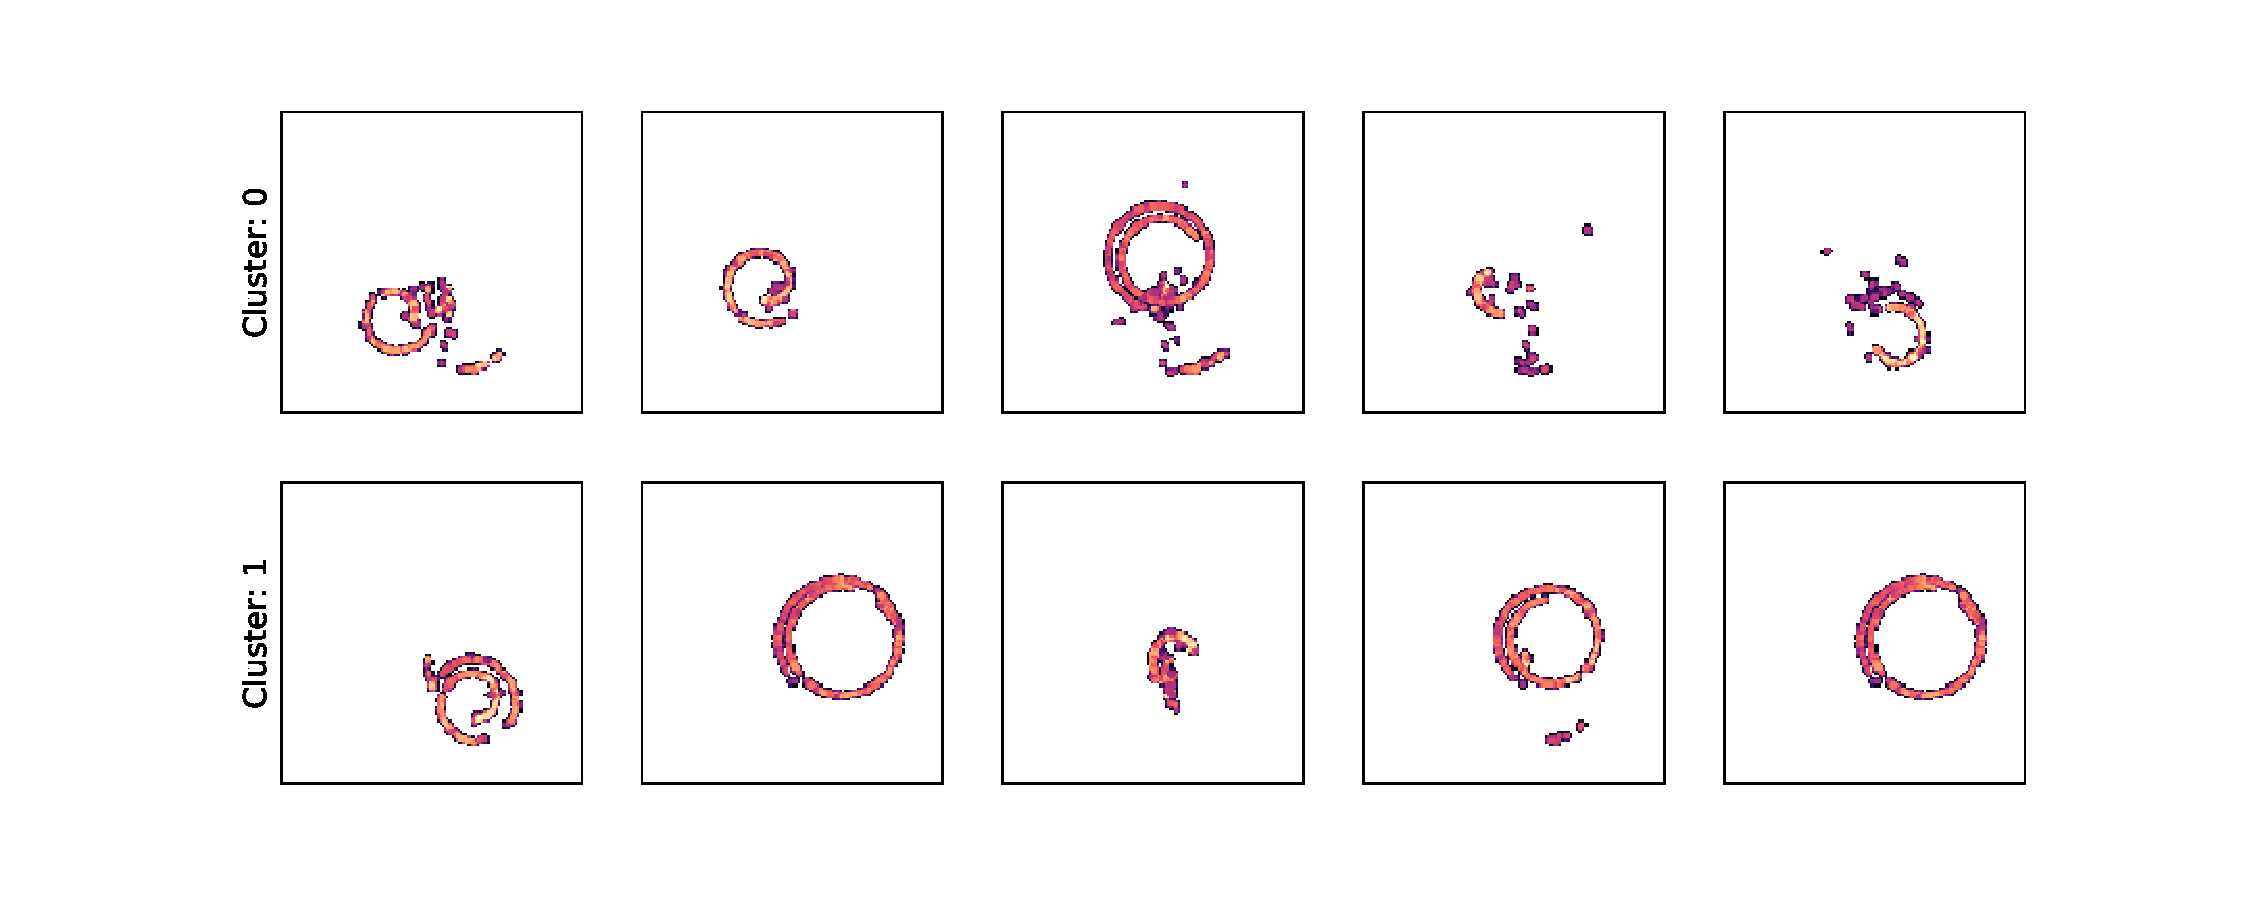
\includegraphics[width=\textwidth]{plots/clean_cluster_repr.pdf}
\caption[Selection of carbon events in differing clusters]{Selection of carbon events belonging to different clusters. Each row represents one of the clusters for the filtered data as shown in figure \ref{fig:mixae_confmat}. There seems to be no clear distinction between these rows.}\label{fig:filtered_mixae_clster_repr}	
\end{figure} 

\begin{figure}
\centering
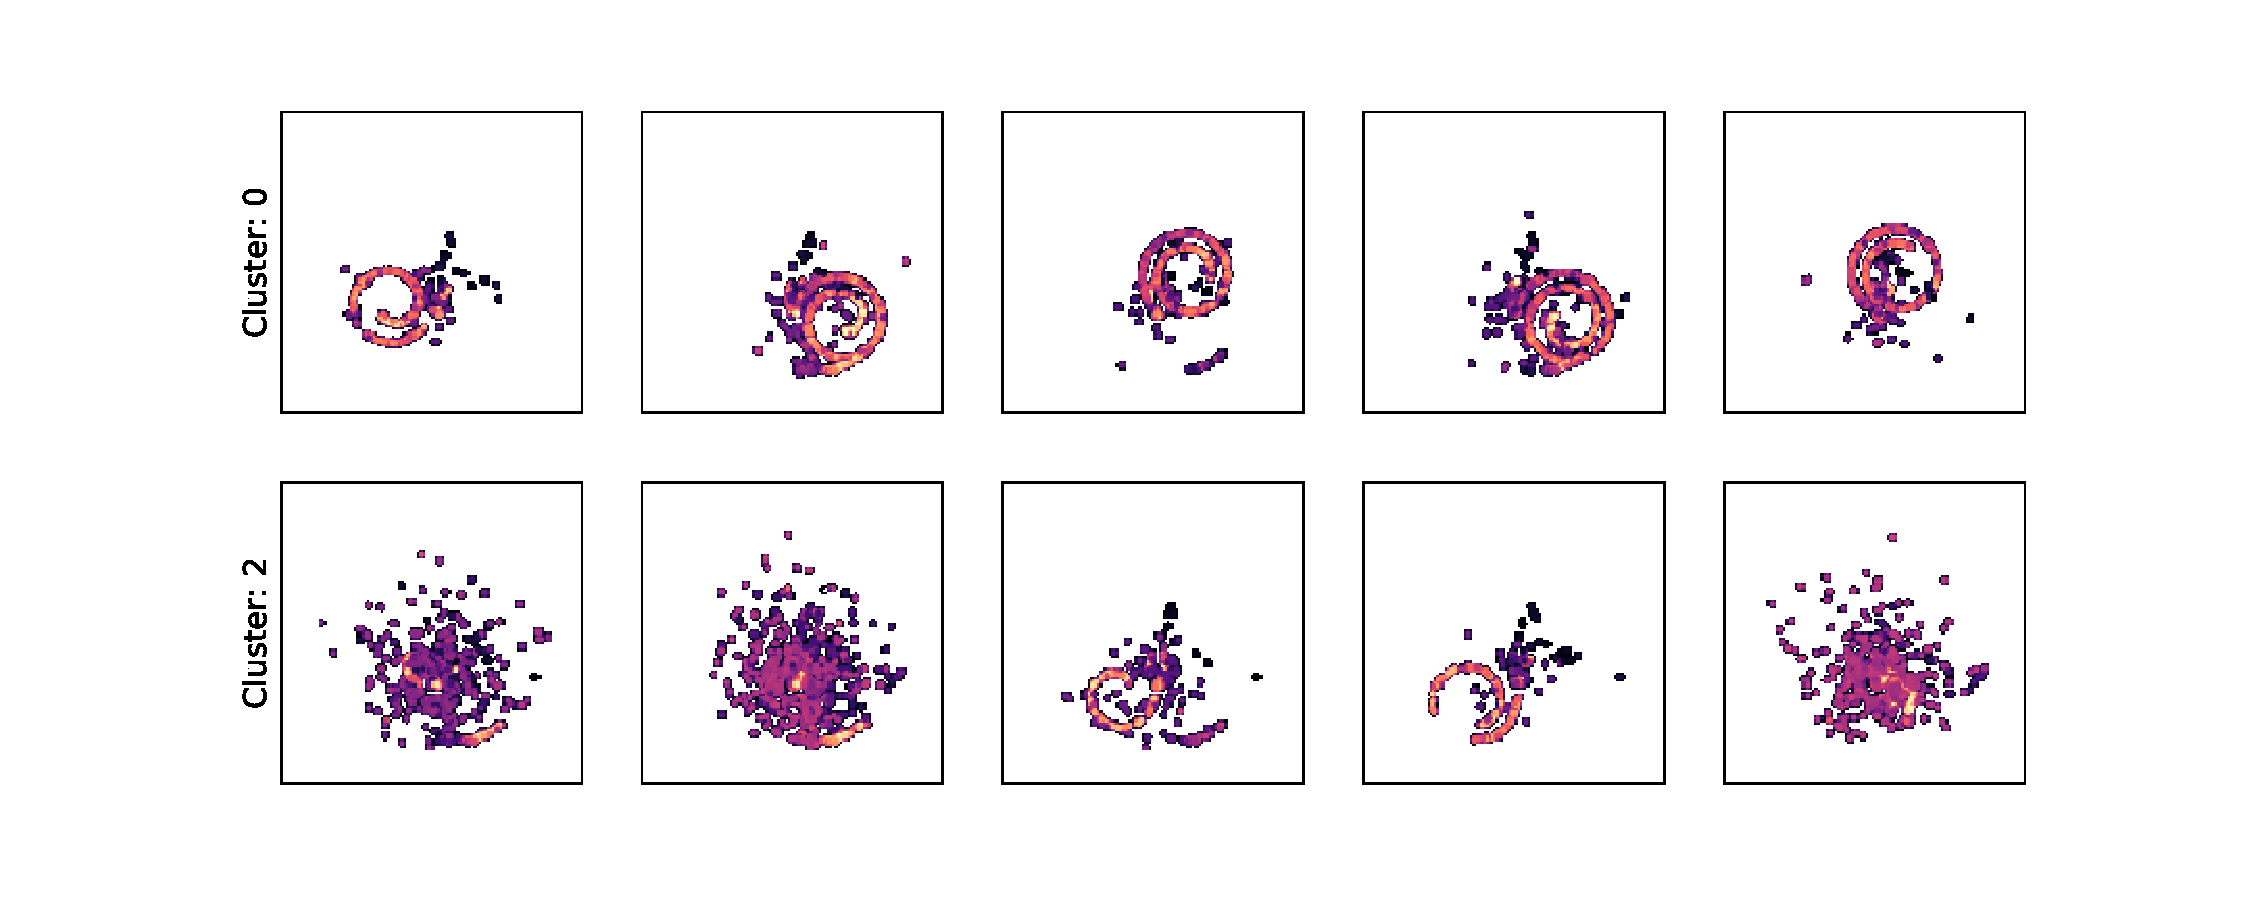
\includegraphics[width=\textwidth]{plots/real_cluster_repr.pdf}	
\caption[Selection of proton events in differing clusters]{Selection of proton events belonging to different clusters. Each row represents one of the clusters for the full data as shown in figure \ref{fig:mixae_confmat}. We observe a tendency for the more noisy events to be placed in the "other" cluster}\label{fig:full_mixae_clster_repr}	
\end{figure} 

\section{Conclusions and Perspectives}\label{sec{conclusion}}

\appendix  
\section{Neural network architectures}

\begin{table}
\caption[vgg architectures]{Showing the details of the VGG network architectures. Network D trained on the ImageNet \cite{Russakovsky2015} dataset the network known as  VGG16 and is what we use in this thesis.}\label{tab:vgg}
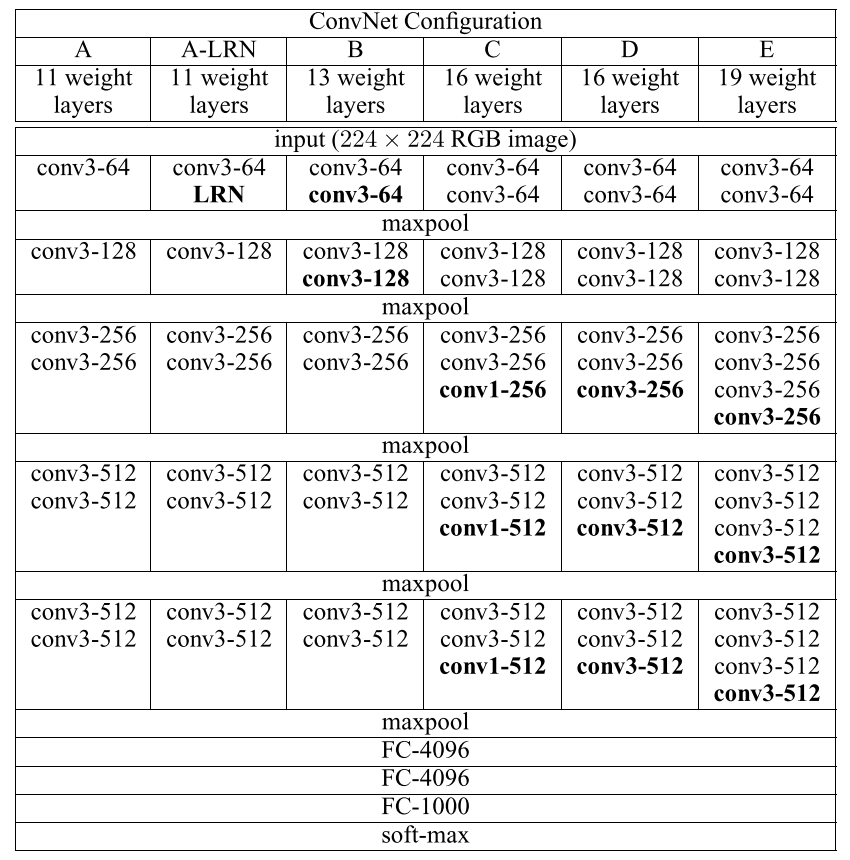
\includegraphics[width=\textwidth]{plots/vgg_architectures.png}
\end{table}

\bibliography{bibliography}
\end{document}
